\newcommand{\svcourse}{CST Part IA: Introduction to Probability}
\newcommand{\svnumber}{1}
\newcommand{\svvenue}{Churchill, Room TBD}
\newcommand{\svdate}{2022-05-14}
\newcommand{\svtime}{11:00}
\newcommand{\svuploadkey}{PO5ogKIM8KQA22FZS8IAf8gxA8XKi19jxIBVHIfFZ+3GCBXuNUXS9lVN6bNYjxM/}

\newcommand{\svrname}{Mr Matthew Ireland}
\newcommand{\jkfside}{twoside}
\newcommand{\jkfhanded}{right}

\newcommand{\studentname}{Harry Langford}
\newcommand{\studentemail}{hjel2@cam.ac.uk}


\documentclass[10pt,\jkfside,a4paper]{article}

\input{../../template/includes.tex}
% DO NOT add \usepackage commands here.  Place any custom commands
% into your SV work files.  Anything in the template directory is
% likely to be overwritten!

\usepackage{fancyhdr}

\usepackage{lastpage}       % ``n of m'' page numbering
\usepackage{lscape}         % Makes landscape easier

\usepackage{verbatim}       % Verbatim blocks
\usepackage{epsfig}         % Embed encapsulated postscript
\usepackage{array}          % Array environment
\usepackage[nolinks]{qrcode}         % QR codes
\usepackage{enumitem}       % Required by Tom Johnson's exam question header

\usepackage{hhline}         % Horizontal lines in tables
\usepackage{siunitx}        % Correct spacing of units
\usepackage{amsmath}        % American Mathematical Society
\usepackage{amssymb}        % Maths symbols
\usepackage{amsthm}         % Theorems

\usepackage{ifthen}         % Conditional processing in tex

\usepackage[top=3cm,
            bottom=3cm,
            inner=2cm,
            outer=5cm]{geometry}

% PDF metadata + URL formatting
\usepackage[
            pdfauthor={\studentname},
            pdftitle={\svcourse, SV \svnumber},
            pdfsubject={},
            pdfkeywords={9d2547b00aba40b58fa0378774f72ee6},
            pdfproducer={},
            pdfcreator={},
            hidelinks]{hyperref}

\renewcommand{\headrulewidth}{0.4pt}
\renewcommand{\footrulewidth}{0.4pt}
\fancyheadoffset[LO,LE,RO,RE]{0pt}
\fancyfootoffset[LO,LE,RO,RE]{0pt}
\pagestyle{fancy}
\fancyhead{}
\fancyhead[LO,RE]{{\bfseries \studentname}\\\studentemail}
\fancyhead[RO,LE]{{\bfseries \svcourse, SV~\svnumber}\\\svdate\ \svtime, \svvenue}
\fancyfoot{}
\fancyfoot[LO,RE]{For: \svrname}
\fancyfoot[RO,LE]{\today\hspace{1cm}\thepage\ / \pageref{LastPage}}
\fancyfoot[C]{\qrcode[height=0.8cm]{\svuploadkey}}
\setlength{\headheight}{22.55pt}

\ifthenelse{\equal{\jkfside}{oneside}}{

 \ifthenelse{\equal{\jkfhanded}{left}}{
  % 1. Left-handed marker, one-sided printing or e-marking, use oneside and...
  \evensidemargin=\oddsidemargin
  \oddsidemargin=73pt
  \setlength{\marginparwidth}{111pt}
  \setlength{\marginparsep}{-\marginparsep}
  \addtolength{\marginparsep}{-\textwidth}
  \addtolength{\marginparsep}{-\marginparwidth}
 }{
  % 2. Right-handed marker, one-sided printing or e-marking, use oneside.
  \setlength{\marginparwidth}{111pt}
 }

}{
 % 3. Alternating margins, two-sided printing, use twoside.
}

\setlength{\parindent}{0em}
\addtolength{\parskip}{1ex}

% Exam question headings, labels and sensible layout (courtesy of Tom Johnson)
\setlist{parsep=\parskip, listparindent=\parindent}
\newcommand{\examhead}[3]{\section{#1 Paper #2 Question #3}}
\newenvironment{examquestion}[3]{
    \examhead{#1}{#2}{#3}\setlist[enumerate, 1]{label=(\alph*)}\setlist[enumerate, 2]{label=(\roman*)}
    \marginpar{\qrcode{https://www.cl.cam.ac.uk/teaching/exams/pastpapers/y#1p#2q#3.pdf}}
    \marginpar{\footnotesize \url{https://www.cl.cam.ac.uk/teaching/exams/pastpapers/y#1p#2q#3.pdf}}
}{}



\usepackage{listings}
\usepackage{tikz}
\usepackage{hyperref}
\usepackage{graphicx}
\graphicspath{ {./images/}}

\begin{document}

\begin{enumerate}

\item A directed graph of n nodes numbered $1, 2, \dots , n$ can be represented by an $n \times n$ 
adjacency matrix $G_1$, where $G_1[i,j]$ is true if there is an edge connecting node $i$ to node $j$, 
and $G_1[i, j]$ is false otherwise.
By extension, define $G_k$ to be that matrix such that $G_k[i, j]$ is true if there is a path of length 
$\leq k$ connecting node $i$ to node $j$, and $G_k[i, j]$ is false otherwise.

Describe an algorithm to generate $G_2$ from $G_1$.

If we consider $G$ to be \textbf{boolean} matrices then we can generate $G_2$ by considering all the 
matrix which is reachable in two steps or one or the 

\begin{equation}
G_2 = G_1 \times G_1 + G_1 \\
\end{equation}

In fact there is a general formula for this:
\begin{equation}
G_{k + 1} = G_1 \times G_k + G_1 \\
\end{equation}

Here is code to calculate which nodes are reachable with a path of $\leq k$.

\begin{lstlisting}[language=java]
public class BooleanMatrix {

    final boolean[][] matrix;

    public BooleanMatrix(boolean[][] matrix) {
        assert (matrix.length == matrix[0].length);
        this.matrix = matrix.clone();
    }

    public boolean[][] k_reachable(int k) {
        boolean[][] nth = matrix.clone();
        boolean changed = true;
        for (int x = 1; changed && (x < k); x++) {
	    /*
	    Note changed is in the termination condition for the 
	    for loop -- so the algorithm terminates if no new paths 
	    are found.
	    */
            changed = false;
            for (int i = 0; i < matrix.length; i++) {
                for (int j = 0; j < matrix.length; j++) {
                    if (i != j) {
                        for (int m = 0; m < matrix.length; m++) {
                            if (matrix[j][m] && nth[m][i]) {
			    // taking the logical or
                                changed = true;
                                nth[j][i] = true;
                                break;
        }}}}}}
        return nth;
}}
\end{lstlisting}

Note that due to the definition of $G_1$ I have assumed that we are do not consider 
zero-length paths as paths.

\item How could this algorithm be used to generate the transitive closure of a graph given its 
adjacency matrix?

If the graph has $n$ nodes then the longest path through the graph which does not visit nodes 
multiple times must have length $n$. So the transitive closure of a graph is the same as the 
matrix $G_n$.

We can calculate $G_n$ (the transitive closure of the graph) by calling k\_reachable with 
argument matrix.length.

\item What is the cost of this transitive closure algorithm in terms of $n$ and $m$, where m is the 
maximum path length in the transitive closure?

My (and the na\"ive) implementation has complexity $\Theta(mn^3)$.

However, there are matrix multiplication algorithms with a better complexity than $\Theta(n^3)$ which 
could lead to a better complexity of this algorithm. However they are far more complicated and have 
high constant factors. If we were to use Strassen's first algorithm for matrix multiplication then 
we would get a complexity of $\Theta(nm^{\lg 7})$ -- even newer algorithms could get 
lower complexites (with even less practical constant factors).

\item Why does Dijkstra's algorithm require non-negative edge weights?

Negative edge weights can cause Djikstra's Algorithm to start cycling infinitely.

\item Would Dijkstra's algorithm work if the only negative weights were on edges leaving 
the source?

As with other graphs with negative edge weights: Djikstra's algorithm would not necessarily work. 
If you cannot reach the source again or the cost of reaching the source is $\geq 0$ then the 
algorithm would work. Otherwise it would loop infinitely.

\item Consider the following approach for finding shortest paths in the presence of negative edges. 
``Make all the edge weights positive by adding a sufficiently large biasing constant to each; then 
find the shortest paths using Dijkstra's algorithm and recompute their weights on the original graph.'' 
Will this work? Justify your answer with a proof or counterexample.

This will not work. I will give a minimal counterexample which has a negative-weight edge cycle.

\begin{center}
\begin{tikzpicture}
\draw (0, 0) circle (0.25);
\draw (3, 0) circle (0.25);
\node (A) at (0, 0) {$\alpha$};
\node (B) at (3, 0) {$\beta$};
\draw [-stealth] (A) to [loop right, out=45, in=135, looseness=1] (B);
\draw [-stealth] (B) to [loop left, out=225, in=315, looseness=1] (A);
\node [anchor=center] at (1.5, 1) {$1$};
\node [anchor=center] at (1.5, -1) {$-2$};
\end{tikzpicture}
\end{center}

Assume we wish to find the shortest path from $\alpha$ to $\beta$. We can clearly see that there is 
no such shortest path -- we can simply go round once more and will obtain a path which is one shorter.

I will add a biasing constant of 3 so that every weight is positive.

\begin{center}
\begin{tikzpicture}
\draw (0, 0) circle (0.25);
\draw (3, 0) circle (0.25);
\node (A) at (0, 0) {$\alpha$};
\node (B) at (3, 0) {$\beta$};
\draw [-stealth] (A) to [loop right, out=45, in=135, looseness=1] (B);
\draw [-stealth] (B) to [loop left, out=225, in=315, looseness=1] (A);
\node [anchor=center] at (1.5, 1) {$4$};
\node [anchor=center] at (1.5, -1) {$1$};
\end{tikzpicture}
\end{center}

In this case we see that the shortest path from $\alpha$ to $\beta$ is 4. We now subtract the 
biasing constant (once since we only went along one edge) and find that the ``true'' shortest path 
from $\alpha$ to $\beta$ has cost 1. However, from the original graph we know there is no shortest path 
and can find an infinitude of counterexamples which have a lower weight: say 
$\alpha \stackrel{1}{\longrightarrow} \beta \stackrel{-2}{\longrightarrow} \alpha \stackrel{1}{\longrightarrow} \beta$ 
which has cost 0.

\item Describe and justify Kruskal’s algorithm for finding the minimum spanning tree of an 
undirected graph.

Given all the edge weights in a graph, keep adding the smallest edge to the minimum spanning tree 
unless the edge connects two nodes both of which are already in the minimum spanning tree. 
This requires $\Theta(E \lg E)$ time.

Firstly, I will prove that the shortest node connecting two otherwise unconnected nodes is a subset of a 
MST then I will prove by induction that repeatedly adding these nodes forms the MST.

Consider a partition $P$ of a MST of the graph $G$.\\
Next consider a the shortest edge $e \in G/P$ which joins two nodes which 
are not otherwise connected call these nodes $V_1$ and $V_2$.\\
Now consider a subset $S$ of the MST which is a superset of $P$ and 
partitions the graph into two sections such that $V_1$ and $V_2$ 
are still not connected and $e$ is not in the subset. \\
Note that $P \subseteq S \Longrightarrow G/S \subseteq G/P$.

By assumption $e$ was the shortest graph in the edges not in the 
partition $P$. Since the $e$ was the shortest edge in in $G/P$, and $G/S \subseteq G/P$, 
$e$ must also be the shortest edge in $G/P$. So since $e$ is the 
shortest edge in $G/P$, there can be no path in $G/S$ which joins 
$V_1$ and $V_2$ which is shorter than $e$. So $e$ must be in the MST.

Hence ``$e$ is the shortest node which connects two otherwise unconnected nodes'' $\Longrightarrow$ $e \in \text{MST}(G)$.

I will prove by induction that after adding $n$ edges this way when $n \leq |G| - 1$, the set of edges we have added is a 
subset of a MST.

After adding 0 edges the set of edges we have added is $\emptyset$ which is a subset of the MST.

If the set of edges after $k$ iterations is $S$ and $S$ is a subset of the MST, then by 
the proof above, if $S \neq \text{MST}(G)$ then adding another edge will mean $S$ is still a subset of the MST. 
Note that |MST| = $n - 1$. So we terminate after inserting $n - 1$ edges.

So since $\emptyset$ is a subset of the MST and adding an edge keeps $S$ a subset of the MST until $S = \text{MST}(G)$, 
we can conclude repeatedly adding the shortest edge which connects two unconnected vertices will form the MST.

This concludes my proof of Kruskal’s algorithm.

\item Consider the problem of finding a minimum spanning tree for 1,000,000 points in a plane 
rectangle where there is an edge between every pair of points and the cost of the edge is the 
Euclidean distance between the two points. What's the best way to find a minimum spanning tree?

There are three sections of my answer to this question:
\begin{itemize}

\item Proof of validity of using a Delaunay Triangulation to form a MST

\item Simple $\Theta(n\lg n)$ algorithm using a Delaunay Triangulation and Kruskal’s algorithm.

\item Optimal $O(n\mathcal{H} + n\alpha(n))$ algorithm.

Unfortunately the worst-case complexity is still $O(n \lg n)$ -- however unlike the 
other algorithms the best-case is $O(n\alpha(n))$.

\end{itemize}

\begin{enumerate}

\item Proofs of validity:

Property 1:\\
If a circle passing through two of the input points doesn't contain any other input points 
in its interior, then the segment connecting the two points is an edge of a Delaunay 
triangulation of the given points \cite{wikipedia}.

Property 2:\\
The number of edges for a Delaunay Triangulation of a graph with $n$ nodes is 
$3n - 3 - h$ where $h$ is the number of edges in the convex hull ($0 < h \leq n$).

Theorem 3:\\
The minimum spanning tree is a subgraph of the Delaunay Triangulation of a set of points.

In the following proof let MST$(V)$ be the minimum spanning tree of the vertices $V$ and DT$(V)$ 
be the Delaunay Triangulation of the vertices $V$.

Proof of Propery 3:\\
Take an arbitrary edge $e \in \text{MST}(V)$ which connects two vertices $V_1$, $V_2$. 
This is the shortest edge connecting two partitions of the vertices. Since there is no 
closer point between the two subsets, there cannot be a vertex within the circle with 
diameter $e$ passing through $V_1$ and $V_2$ (else the distance to one of the nodes from 
the other partition would be less than $|e|$ and $e \notin \text{MST}$ as assumed). So by 
Property 1, edge $e$ must be in DT$(V)$. This means that the Minimum Spanning Tree of a 
graph is a subgraph of the Delaunay Triangulation of the same graph.

This proves $e \in \text{MST}(V) \Longrightarrow e \in \text{DT}(V)$. So finding the Minimum 
Spanning Tree of a Delaunay Triangulation of a graph is the same as the Minimum Spanning 
Tree of the complete graph.

\item The first algorithm is simple:

\begin{itemize}

\item Use a divide-and-conquer algorithm to make the Delaunay Triangulation in $\Theta(n\lg n)$ time.

\item Use Kruskal's algorithm to build the Minimum Spanning Tree from the Delaunay Triangulation 
in $\Theta(E \lg V)$ time where $E < 3n - 3$, $V = n$. This is $\Theta(n \lg n)$ time.

\end{itemize}

Get the delauney triangulation using the divide-and-conquer method. This takes $\Theta(n \lg n)$ 
time \cite{nlgndelaunay}. The number of adjacent nodes in a delauney triangulation is known to be bounded by a constant for a 
set of points on a 2D plane. We now have $kn$ edges where $k$ is a constant. We then use Kruskal’s algorithm to build 
a minimum spanning tree from the delauney triangulation $\Theta((V + E) \lg V)$ time. Since $E < 3V$ and $V = n$ this is 
$\Theta(n\lg n)$. We have now build a minimum spanning tree of the poins in $\Theta(n \lg n)$ time.

\item The summary for the optimal algorithm is as follows:

\begin{itemize}

\item Sort the vertices by an arbitrary coordinate ($z$) using a TimSort-like algorithm \cite{shiverssort} with a 
complexity of $\Theta(n + n\mathcal{H})$ \cite{timsortcomplexity} or Radixsort if $z$ coordinates are integral.

\item Use a sweep-line algorithm to build a simple polygon from the sorted points in linear time.

\item Use the linear time algorithm to make a delaunay triangulation from a simple polygon \cite{lineardelaunay}.

\item Use an asymtotically optimal MST algorithm to make a MST from the dalaunay triangulation in $O(n\alpha(n))$ \cite{optimalmst}.

\end{itemize}

This algorithm is dominated by the initial cost of sorting the points which are passed to it.

This algorithm achieves near-linear complexity if the points passed to it 
are sorted (or almost sorted) by $z$ coordinate. The following algorithm has a 
complexity of $O(n\mathcal{H} + n\alpha(n))$ where $\mathcal{H}$ is the 
entropy of the distribution of the length of ordered runs in $x$ coordinates of the 
vertices and $\alpha$ is the inverse ackermann function.

Note that for all inputs $\mathcal{H} \in O(\lg n)$ however if the input vertices are 
sorted or almost sorted by $x$ coordinate then $\mathcal{H} \in O(1)$. This means that on some 
inputs this algorithm will have a complexity of $\Theta(n\alpha(n))$. 

Sort nodes by a coordinate $x$ subsorted by $y$ using a ``Timsort-like'' algorithm. This is the 
informal name for ``k-aware merge-sort algorithms'': these algorithms are 
more advanced versions of mergesort which are able to take advantage of partial order within 
lists to reduce the number of comparisons they make -- Timsort is the most common however there are others 
which have a constant lower number of required comparisons. The expected cost of this sort is
$\Theta(n + n\mathcal{H})$. Note that if vertices are sorted or near-sorted by $x$ then this is linear.

Use a sweep-line algorithm to build a simple-polygon from the set of points.

The below algorithm takes a sorted list of distinct points and passes through it once building a 
simple polygon by repeated insertion. The insertion is constant time since the points are sorted and 
so the overall complexity of this algorithm is $\Theta(n)$.

The algorithm maintains two invariants: 
\begin{itemize}

\item ``rightmost'' is the point we have seen with the highest $x$ coordinate

\item rightmost.left.y() > rightmost.right.y()

\end{itemize}

\begin{lstlisting}[language=python]
class Vertex:
    def __init__(self, x, y):
        self.__x = x
        self.__y = y
        self.left = None
        self.right = None

    def __repr__(self):
        return "(" + str(self.__x) + " " +  str(self.__y) + ")"

    def x(self):
        return self.__x

    def y(self):
        return self.__y


def sweep_polygon(vertices: list[tuple[float, float]]):
    # base case builds a single triangle.
    # If this cannot be done then the input size
    # is < 3 so building the MST is constant time
    v0 = Vertex(vertices[0][0], vertices[0][1])
    v1 = Vertex(vertices[1][0], vertices[1][1])
    v2 = Vertex(vertices[2][0], vertices[2][1])
    if v0.y() < v1.y():
        v2.right = v0
        v2.left = v1
        v1.right = v2
        v1.left = v0
        v0.right = v1
        v0.left = v2
    else:
        v2.right = v1
        v2.left = v0
        v1.right = v0
        v1.left = v2
        v0.right = v2
        v0.left = v1
    rightmost = v2
    for vertex in vertices[3:]:
        v = Vertex(vertex[0], vertex[1])
        if rightmost.x() == v.x():
            rightmost.left.right = v
            v.left = rightmost.left
            rightmost.left = v
            v.right = rightmost
            rightmost = v
            continue
        gradient_a = (v.y() - rightmost.y()) / (
		v.x() - rightmost.x())
        gradient_right = (v.y() - rightmost.right.y()) / (
		v.x() - rightmost.right.x())
        if gradient_a < gradient_right:
            rightmost.right.left = v
            v.right = rightmost.right
            rightmost.right = v
            v.left = rightmost
        else:
            rightmost.left.right = v
            v.left = rightmost.left
            rightmost.left = v
            v.right = rightmost
        rightmost = v
    return rightmost
\end{lstlisting}

This algorithm produces simple polygons from any set of points as shown below
\begin{center}
\includegraphics[width=5cm]{polygon}
\end{center}

Note that this specific implementation assumes points are distinct. Given that we are considering points on a 
euclidean plane which are only distinguishable by their coordinates, if two vertices are passed with the same 
coordinate then we can consider them as a single vertex and will get the same MST at the end. Less elegant 
implementations can be made which deal with duplicate points either by inserting them at the end or keeping two 
rightmost nodes when nodes are the same.

Next use the constrained linear algorithm to make the delauney triangulation from the simple polygon 
in linear time \cite{lineardelaunay}. 

Now we must only build a MST from a Delaunay Triangulation in $o(n\lg n)$ to achieve a better complexity 
than the na\"ive algorithm. This is possible.

There is a linear MST algorithm which can be applied if the graph is sufficiently dense: if 
$\frac{E}{V} \geq \lg \lg \lg V$. Note that for a delaunay triangulation, 
$\frac{E}{V} = \frac{3n - 3 - h}{n} \geq 2 - \frac{3}{n}$ and so the density requirement is guaranteed 
for graphs of size $V \leq 65472$. So MST generation algorithm is guaranteed linear for small inputs.

For random graphs, the the expected proportion of nodes in a convex hull is $\tilde n^{-\frac{2}{3}}$ 
\cite{minhull} and so as $n\longrightarrow \inf$, $\frac{E}{V} \longrightarrow 3$. So for most non-adversarial 
graphs of size $< 10^{77}$ the density criteria is met and we can apply the linear-time algorithm. Unfortunately 
this is not guaranteed and so we \textit{may} have to use the optimal superlinear algorithm with complexity 
$O(n\alpha(n))$.

The generalisation of this will run the Petitte and Ramachandran's provably optimal function. This has 
a complexity of $\Omega(V)$ and $O(E\alpha(E, V))$. Since we have bounded $E$ to $V \leq E < 3V$ and $V = n$, 
we have that the complexity of building the MST from the Delaunay Triangulation is $\Omega(V)$ and $O(V\alpha(V))$

So the overall complexity of the algorithm is $O(n\mathcal{H} + n\alpha(n))$.

\end{enumerate}

\end{enumerate}

\bibliographystyle{ieeetr}
\bibliography{citation}

\end{document}